\chapter{Ap�ndice}\label{ape:a}

Anexo Modelo de Acordo de N�vel de Servi�o.

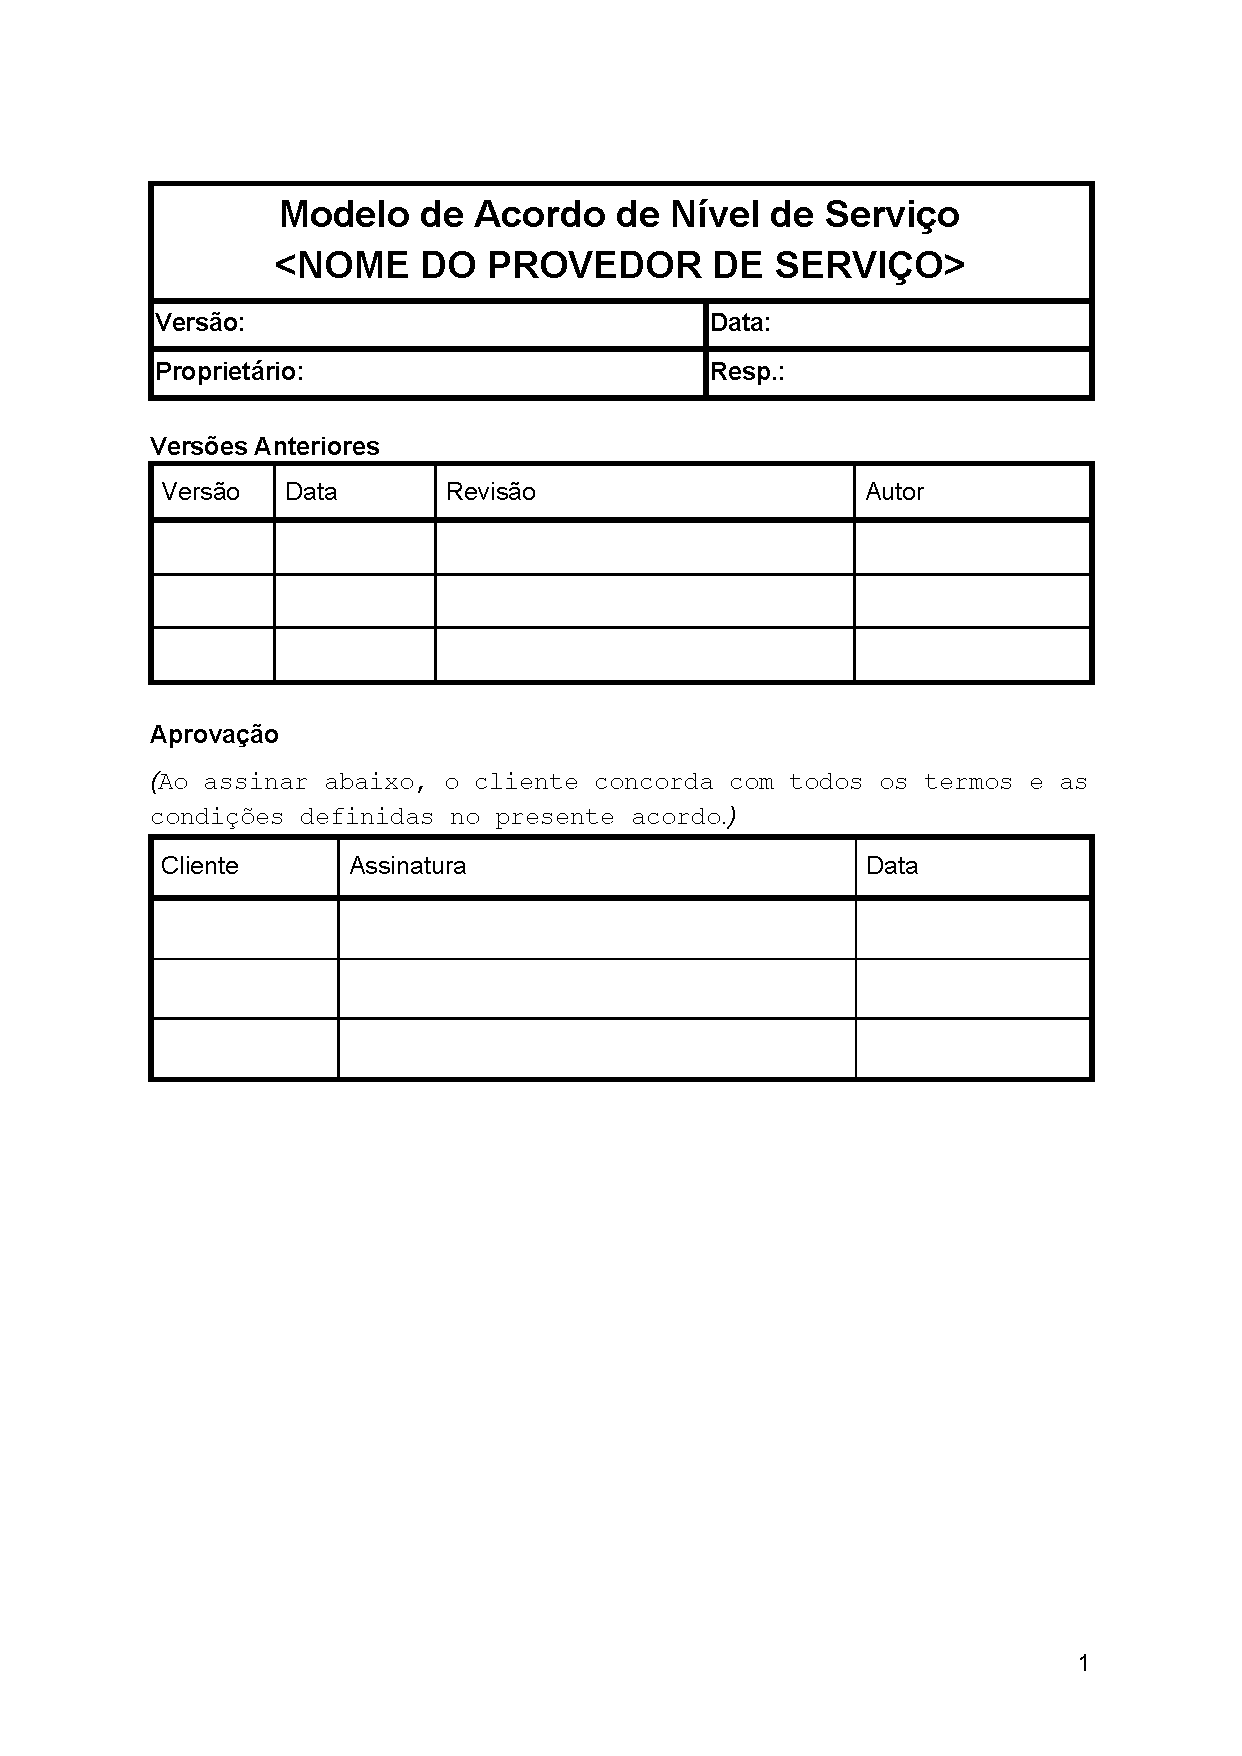
\includepdf[pages=-,pagecommand={},width=\textwidth]{./mods/modelo-de-ANS.pdf}

%\chapter{Ap�ndice}\label{ape:b}
%
%Semelhante ao ap�ndice anterior, cada p�gina desse ap�ndice contem uma tabela de m�tricas em sua vers�o absoluta e relativa de relacionamento entre os desenvolvedores. Os desenvolvedores est�o dispostos nas linhas e colunas formando a matriz de relacionamento. Para interpreta��o dos resultados, deve-se considerar os desenvolvedores das colunas como agentes de munda�a nos desenvolvedores das linhas, ou seja, os desenvolvedores dispostos nas linhas sofreram altera��es do desenvolvedores que est�o dispostos nas colunas. Ao final, todas as m�tricas que foram formalizadas no Cap�tulo \ref{cap:metricas} s�o apresentadas para o projeto Solicite. Na sequ�ncia, existe tamb�m, uma tabela de tr�s p�ginas que revela o valor das m�tricas de todos os desenvolvedores. Dessa vez, os desenvolvedores est�o disposto nas linhas e as colunas correspondem as m�tricas.
%
%\includepdf[scale=1,offset={0 -70}]{apendices/solicite_stats_authors.pdf}
%\includepdf[scale=1,offset={0 -70}]{apendices/solicite_metrics_all.pdf}

